\subsection*{Historical alternative-model follow-up, 13 October 2026}
This earlier checkpoint is retained to explain failed approaches. The current authorized-grid run is reported in its own section; the paragraphs here do not describe its completion status.
The frozen calibration cohort contains 1,003 provisional associations. Its event identifiers and earlier magnitude, template and frequency-index products are preserved. An additional 43 successful six-hour waveform requests supplied 525,189,120 bytes and 703.785 channel-hours; 5 requests returned HTTP 204. The segmented queue now has 694 successful requests, 34 no-data responses and 73,946 unattempted requests. Pending intervals remain unfinished acquisition, not evidence of remote inaccessibility.

The separate expanded checkpoint processed 868 files from 26 station names, with 8511.520 union channel-hours. It produced 132,733 merged picks (19,530 P and 113,203 S), and 1,015 provisional associations containing 7,351 assigned picks. These identifiers are not interchanged with the earlier calibration cohort. Complete epoch intersections identify 0.000 channel-hours without a usable saved response. This checks metadata availability, not response accuracy or complete three-component detection exposure. Station coverage, every unobserved interval and request status are saved under \path{data/calibration_followup/expanded}. No expanded event is yet promoted to an accepted location or substituted into earlier magnitude plots.

\paragraph{Executed VELEST chain.}
The written methods identify 373 high-quality calibration events but give no numerical rule that uniquely selects them. The declared causality, more-than-six-pick and gap-below-$180^\circ$ screen selects 130 events: 24, 1, 1, 104 in 2022--2025. 3 have only S picks. This is an unreviewed and temporally unrepresentative alternative selection. The starting layers are Tramelli et al. (2021), Table 1, with the top extended to $-0.5$ km for station elevations. They are not the missing Battaglia regional averages. The reference P delay at IV.CSOB. is fixed; initial delays are zero. Two calibration rounds estimate locations/velocities and then also station delays, using seven iterations per round and the preceding explicit damping and S/P weights.

Both arithmetic precisions completed both rounds. The fitted velocity tables agree at their printed precision; maximum location differences are 11.105 m horizontally and 10.0 m vertically. Five fixed-model, fixed-correction catalog passes were executed on 905 causally consistent candidates, including the stated 0.4 s and 0.3 s residual rejection. The final six-pick, 0.25 s and $300^\circ$ filters retain 238 exploratory locations. Fixed models/corrections were checked after every pass; absolute own-pick times were preserved to 0.001609 s through serialized origin-time changes.

\paragraph{Validation rejects acceptance.}
Another five seven-iteration passes do not converge. The last moves an event by 4.935 km horizontally and 2.04 km vertically; a fitted depth reaches 18.40 km. These are unstable trial estimates, not newly established deep earthquakes. With every fifth chronological event held out, unweighted phase RMS worsens from 0.314 to 0.385 s, although aggregate reported event RMS changes from 0.335 to 0.319 s. Recalculation shows that VELEST reports a sample standard deviation of normalized weighted residuals rather than unweighted phase RMS. Maximum discrepancy from the printed values is 0.005221 s, consistent with output rounding. Thus the mixed validation is not resolved by relabeling both metrics RMS.

One declared sensitivity trial requires at least four P and two S picks and excludes initial depth-bound hits. It leaves 46 events. Further iterations produce $V_p\leq V_s$; its held-out training branch also fails that physical check. Neither fit is propagated. Reviewed phase identities and well-constrained events are needed before another regional fit can be accepted. The stationary-coordinate approximation differs from sampled channel epochs by up to 12.990 m, already relevant to a claimed ten-meter precision. These checks establish reasons for rejection, not an accepted calibrated catalog.

\begin{figure}[H]\centering
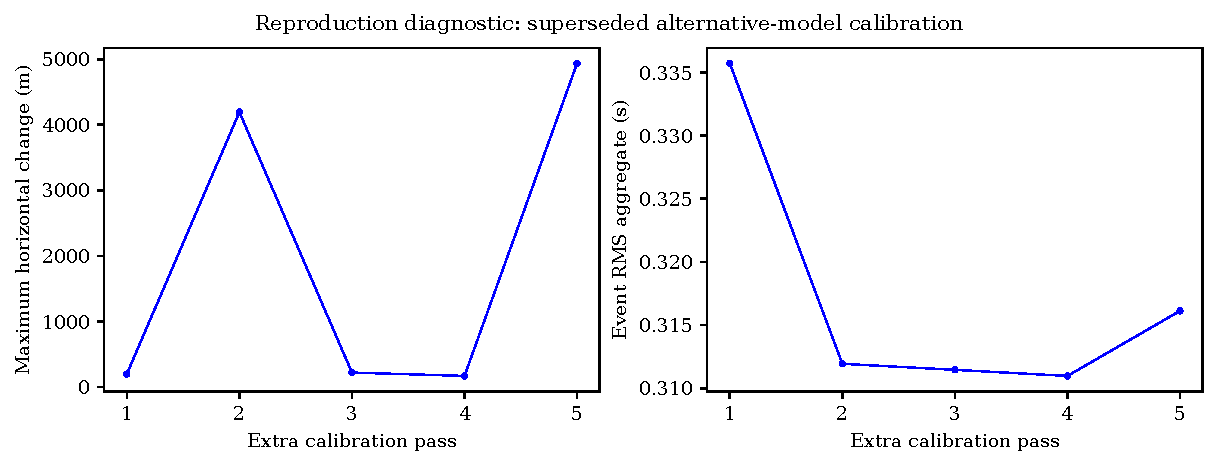
\includegraphics[width=.96\linewidth]{figures/calibration_convergence_diagnostic.pdf}
\caption{Reproduction diagnostic, not a publication figure. Saved convergence trials show kilometer-scale location changes despite similar residual statistics. The model and locations are rejected for scientific interpretation.}
\end{figure}

\paragraph{Observed delays and exploratory HypoDD.}
The 238-event filtered trial supplies 1653 nearest-neighbor pairs and 6362 catalog differential phases. Original response-corrected waveform measurements supply 10,882 channel comparisons, 737 passing channels and 517 coherency-weighted station/phase delays; 13 window failures are retained. The preceding two-second window, 1--15 Hz band and correlation/coherence thresholds are explicit assumptions, not recovered author configuration. Rejected picks or published event solutions are not used to fill gaps.

Generic HypoDD 2.1 was obtained from Waldhauser's official repository at revision \path{fb40407} (full commit in the source receipt). Bounds checks exposed an incorrect output-vector dummy extent in \path{matmult2.f}; it was changed from the column count to the row count, with unchanged multiplication equations. An isolated synthetic matrix assertion checks that fix and never enters empirical data. Source hashes, dimensions, compiler flags and the exact change are recorded in \path{hypodd21_sources.json} and \path{hypodd_build.json} under the follow-up data directory.

Two alternative-profile HypoDD LSQR rounds returned 127 and 126 locations. These are not TomoDD rounds. Six shared phases link clusters; two four-iteration blocks shift weight from catalog to waveform delays, with LSQR damping 50, and a $300^\circ$ gap ceiling. Magnitudes and initial errors set to zero are unused format fields, not measured quantities. LSQR error columns are not interpreted as uncertainties. Quadrants about $14.14^\circ$E, $40.82^\circ$N provide explicit alternative SVD subsets; they do not recreate the paper's four numerical selections. Smaller underconstrained components failed, so only the largest connected component in each quadrant was attempted. NW, SW and SE return 40, 16, 22 estimates; NE diverges and supplies no valid output. The largest conditional 95\% depth errors are 4494.8, 662.9, 507.7 m, respectively. These conditional errors and unstable locations cannot establish the publication's spatial precision. No S7 panel is promoted.

\begin{figure}[H]\centering
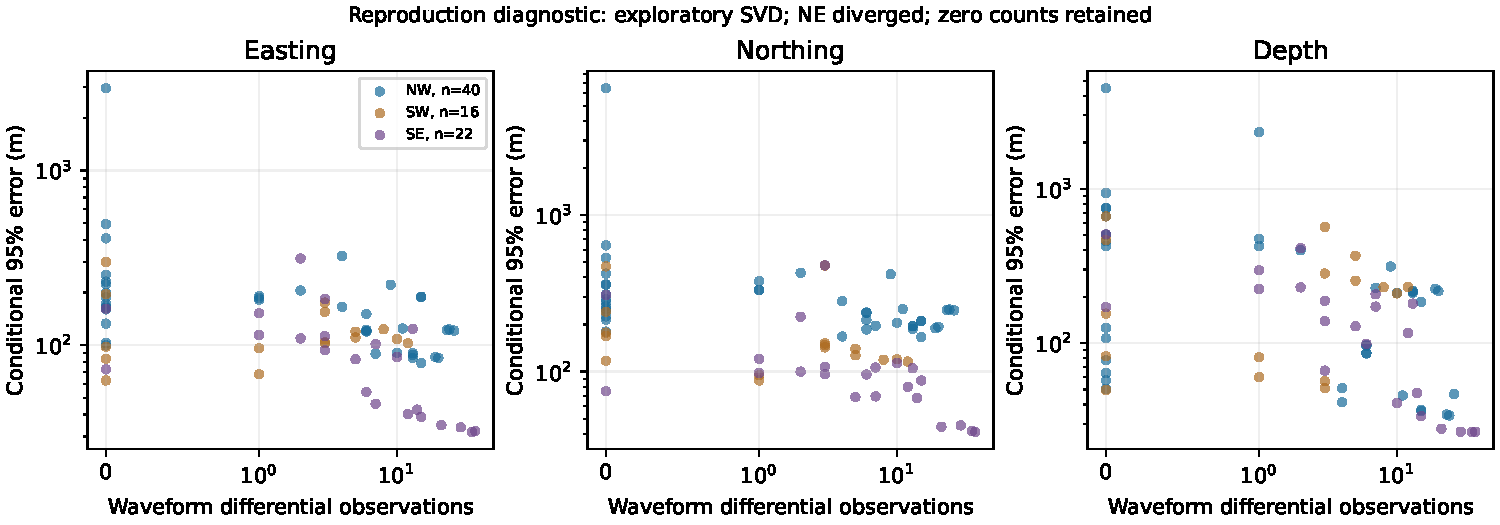
\includegraphics[width=.96\linewidth]{figures/relocation_uncertainty_diagnostic.pdf}
\caption{Reproduction diagnostic, not Figure S7. Conditional SVD errors for three exploratory connected components; the fourth diverged. Zero waveform-difference counts are retained on a symmetric-log abscissa. Error bars cannot validate unreviewed events or the background model.}
\end{figure}

\paragraph{Provenance and remaining prerequisites.}
The authorized De Siena et al. (2017) article cites the original Battaglia model and links PANGAEA 875535. Its inspected metadata list derived locations, attenuation products, geochemistry and map material; no numerical original $V_p/V_s$ grid is identified. Those derived products were not downloaded as analysis inputs. At that checkpoint the model was quarantined. It is now explicitly authorized as a reference input; the new grid-derived results above supersede this historical completion record. Source receipts, URL and hash are recorded; no correspondence was initiated. Exact Cal\`o--Tramelli layer depths and velocities also remain missing, but did not prevent these explicitly alternative trials. TomoDD using the stated fixed 3D background, accepted-location magnitudes, the four specified S7 subsets and their dependent structural panels remain uncompleted. Reviewed phases, stable calibration, verified numerical grid/coordinates/depth convention and regional-averaging masks remain prerequisites. Coverage remains sparse and RAN waveforms credential-gated. Additional observations alone do not resolve the failed calibration.

The complete own-run controls, input serialization, logs and outputs, including failures, are preserved in \path{data/calibration_followup/run_records.zip} with member hashes. Code and commands are in \path{docs/CALIBRATION_FOLLOWUP.md}. The incremental rebuild executes these trials and reports scientific failures separately from successful software execution; it does not claim a full-period reproduction. Earlier magnitude, focal-mechanism and hybrid statuses are unchanged.
